\documentclass[11pt,paper=a4,final]{scrartcl}
\usepackage[utf8]{inputenc}
\usepackage{geometry}           %allows us to specify the 'seitenrand'
\usepackage{graphicx}           %package used to include graphics
\usepackage{hyperref}           %used to make klickable links
\usepackage{listings}
\usepackage{tabularx}
\usepackage{pdflscape}
\usepackage[figuresright]{rotating}
\usepackage{nameref}
\usepackage{longtable}
\usepackage{enumitem}
\usepackage{ngerman} % Make the document German
% Make the document German
\usepackage{ngerman}
\usepackage{fancyhdr}
\usepackage{lipsum}
\usepackage{mdwlist}
\usepackage{multirow}

\hypersetup{
    colorlinks,
    citecolor=black,
    filecolor=black,
    linkcolor=black,
    urlcolor=black
}


\title{Arbeitsjournal}
\author{Niklaus Hofer, Roland Rytz}
\date{\today{}}

% Make title and author accessible in the header/footer
\makeatletter
  \let\Title\@title
  \let\Author\@author
\makeatother

\pagestyle{fancy}

\geometry{a4paper, top=20mm, right=20mm, bottom=30mm, left=20mm}

\fancyhf{}      %delete default values
\setlength{\headwidth}{\textwidth}      %header and footer width equal the text width
\lhead{\Author}
\rhead{\Title}
\fancyfoot[CE,CO]{Speicherdatum: \today{}}
\fancyfoot[RE,RO]{\thepage}

\begin{document}
\maketitle
\newpage
\section{Dokumenteninformationen}
\subsection{\"Anderungskontrolle}
\subsection{Referenzierte Dokumente}
\subsection{Verwendete Abk\"urzungen}
\tableofcontents
\listoffigures
\listoftables
\section{Managementsummary}
\subsection{Aufgabenstellung}
\subsection{Varianten}
\subsection{Konzept}
\subsection{Realisierung}
\subsection{Testbericht}
\subsection{Mittelbedarf}
\subsection{Fazit}
\part{Ablauf und Umfeld}
\section{Projektmethode Hermes}
\begin{figure}[htb!]
  \centering
  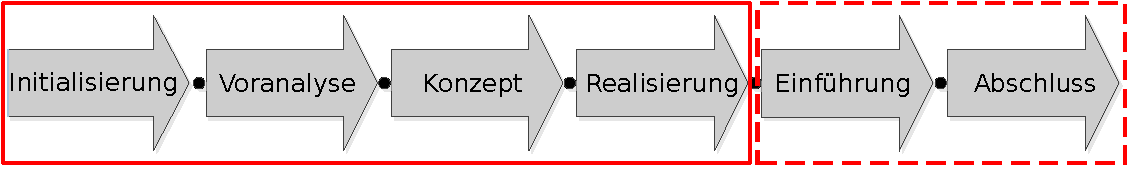
\includegraphics[width=\textwidth]{hermes.pdf}
  \caption{Hermes Light Schema}
  \label{fig:hermes_schema}
\end{figure}
Wir haben die Projektmethode Hermes Light gew\"ahlt. Hermes Light ist eine vereinfachte und verkürzte Variante von Hermes. In der Grafik \ref{fig:hermes_schema} sind die sechs Phasen der Projektmethode aufgezeigt. Die letzten zwei Phasen, \glqq Einführung\grqq und \glqq Abschluss\grqq werden im Rahmen dieser IPA nur teilweise durchgeführt. Die Einf\"uhrung besteht im Bereitstellen der Webseite und des Artikels. Der Abschluss allerdings wird hier nur beschrieben.

In den Abschnitten unten, werden wird die jeweilige Phase kurz erläutern und aufzeigen welche Teile dieses Dokumentes zu welcher Phase gehören.
\newpage
\subsection{Initialisierung}
\begin{itemize}
  \item Festlegung eines klar definierten organisatorischen und technischen Rahmens als Voraussetzung für eine erfolgreiche Projektabwicklung
  \item Planung, Vernehmlassung und Beurteilung des Projekts
  \item Freigabe der Phase Voranalyse
\end{itemize}
Diese Phase beinhaltet folgende Punkte dieser Dokumentation:
% TODO
\begin{itemize}
  \item 
\end{itemize}
\subsection{Voranalyse}
\begin{itemize}
  \item Erstellung und Beurteilung der Situationsanalyse sowie Überprüfung der Zielsetzungen, der Problemstellung und des Untersuchungsbereichs
  \item Erarbeitung von Lösungsvorschlägen und Abschätzung ihrer voraussichtlichen Wirtschaftlichkeit und Realisierbarkeit
  \item Auswahl eines Lösungsvorschlages und Freigabe der Phase Konzept.
\end{itemize}
Diese Phase beinhaltet folgende Punkte dieser Dokumentation:
% TODO
\begin{itemize}
  \item 
\end{itemize}
% TODO
Eigentlich beinhaltet diese Phase noch die Punkte \glqq Termine\grqq und \glqq Zeitplan\grqq . Aufgrund des Ablaufs der IPA und da diese Daten gegeben sind, habe ich oben genannte Punkte aber in die Phase Initialisierung verschoben.
\subsection{Konzept}
\begin{itemize}
  \item Vollständige Darstellung des Systems, ausgehend vom gewählten Lösungsvorschlag
  \item Beurteilung kritischer Teilsysteme
  \item Freigabe der Phase \glqq Realisierung\grqq
\end{itemize}
Diese Phase beinhaltet folgende Punkte dieser Dokumentation:
% TODO
\begin{itemize}
  \item 
\end{itemize}
Die Konzeptphase widmet sich der konkreten Gestaltung des Systems. Es beinhaltet die Struktur, die Architektur, das Design, sowie die Funktionalitäten der zu entwickelnden Applikation.
\subsection{Realisierung}
\begin{itemize}
  \item Erkläuterungen zum geschriebenen Code
  \item Aufzeigen und Begründen von Änderungen gegenüber dem Konzept
  \item Freigabe der Phase Einführung
\end{itemize}
Diese Phase beinhaltet folgende Punkte dieser Dokumentation:
% TODO
\begin{itemize}
  \item 
\end{itemize}
\subsection{Einf\"uhrung}
\subsection{Abschluss}
\section{Aufgabenstellung}
\subsection{Ausgangslage}
\subsection{Auftragsformulierung}
% TODO
% Einfuegen des Auftrages
\subsubsection{Detaillierte Aufgabenstellung}
\subsection{Tests}
\subsection{Mittel und Methoden}
\begin{table}[h!]
 \centering
  \begin{tabular}{|l|p{10cm}|}
  \hline
  Projektmethode & Hermes Light, Eine auf den Projektumfang zugeschnittene Variante von Hermes \\ \hline
  Systeme & Computer zum Schreiben des Codes. Internetanschluss \\ \hline
  Testing environment & System das in der Lage ist, virtuelle Mascheinen auszuf\"uhren zum Testen mit verschiedenen Browsern unter verschiedenen Systemen \\ \hline
  Entwicklungssoftware & Editor, Browser, Javascript, JQuery \\ \hline
  Dokumentation & Texteditor, pdflatex, MikTex \\ \hline
  Entwicklungssprache & Javascript \\ \hline
  Versionsverwaltung & git, github \\ \hline
  \end{tabular}
  \caption{Auflistung der Mittel und Methoden}
\end{table}
\subsection{Projektorganisation}
% TODO
% Grafik erstellen
\subsection{Projektrollen}
\begin{table}[h!]
  \centering
  \begin{tabular}{|l|l|l|}
    \hline
    \bf Funktion & \bf Person & \bf Beschreibung \\ \hline
    Auftraggeber & Herr Tschopp & Lehrkraft \\ \hline
    Projektleiter & Niklaus Hofer & \\ \hline
    Fachberater Mathematik & Herr L\"uthi & Lehrkfraft \\ \hline
    Fachberater Deutsch & Herr Tschopp & Lehrkraft \\ \hline
    Entwickler & Roland Rytz & \\ \hline
    Entwickler & Niklaus Hofer & \\ \hline
  \end{tabular}
\end{table}
\section{Vorkenntnisse}
Roland Rytz ist erfahrener Javascript Entwickler. Im Verlauf seiner Berufslehre
als Informatiker EFZ hat er zahlreiche Webseiten und Webapplikatione mit
Javascript realisiert. Roland hat dann auch in diesem Bereich seine
Abschlussarbeit geschrieben Auch in der Freizeit hat Roland bereits einige
Webseiten geschrieben. JQuery, die Webentwicklungswerkzeuge von Googles Chrome
Browser und Firefox FireBug sind vertraute Werkzeuge. Auch das Testen mit
verschiedenen Browsern ist keine Neuheit.

Niklaus Hofer hat bereits einfache Vigenere Implementationen in C++, Python und
Java geschrieben und sich kurz theoretisch mit dem Thema auseinandergesetzt.

\section{Vorarbeiten}
\section{Termine}
\section{Arbeitsjournal}
\begin{landscape}
  \section{Arbeitsjournal}
  Datum im Format Jahr.Monat.Tag
  \begin{longtable}{|p{1.8cm}|p{1.5cm}|p{5.0cm}|p{11.0cm}|l|l|}
    \hline
    \multirow{2}{*}{\bf Datum} & \multirow{2}{*}{\bf Wer} &\multirow{2}{*}{\bf T\"atigkeit} & \multirow{2}{*}{\bf Reflexion} & \multicolumn{2}{c|}{\bf Zeit} \\ \cline{5-6}
     & & & & \bf Geplant & \bf Effektiv \\ \hline
    %Use the headings below if you don't have multirow installed
    %\bf Datum & \bf Wer & \bf T\"atigkeit & \bf Reflexion & \bf Geplant & \bf Effektiv \\ \hline
    \hline
    \endhead
    % Beginn section ---------------------------------------------------------
    2012.09.09 & Niklaus und Roland &
    Initialisierung des Repositories. &
    Die Zusammenarbeit funktioniert bis jetzt gut. &
    20min & 20min \\ \hline \nopagebreak
    \multicolumn{2}{|l|}{\bf Pendenzen} &\multicolumn{2}{p{16.0cm}|}{Planen des weiteren Vorgehens.}  & \multicolumn{2}{l|}{} \\ \hline
    % End section ------------------------------------------------------------
    % Beginn section ---------------------------------------------------------
    \hline
    2012.10.19 & Niklaus und Roland &
    Schreiben des ersten Programmcodes. Erstellen des Vigenere square mit HTML und Javascript. &
    Der Wiedereinstieg in die Progammierung ist nicht ganz einfahc gefallen. Wir hatten deshalb deutlich l\"anger als urspr\"unglich geplant und sind auch nicht so weit fortgeschritten wie geplant. &
    30min & 80min \\ \hline \nopagebreak
    \multicolumn{2}{|l|}{\bf Pendenzen} &\multicolumn{2}{p{16.0cm}|}{Wir wollen die grundlegenden Funktionen implementieren, damit wir beim ersten Gespr\"ach mit Herr L\"uthi bereits etwas zeigen k\"onnen. Insbesondere die 'sichtbaren' Funktionen sollten dann da sein. Das GUI muss dann aber nat\"urlich noch nicht fertig sein.}  & \multicolumn{2}{l|}{} \\ \hline
    % End section ------------------------------------------------------------
    % Beginn section ---------------------------------------------------------
    \hline
    2012.10.19 & Niklaus &
    Implementieren des Verschl\"usselungsalgorithmus in Javascript. Testen der Verschl\"usselung, Vergleich mit einer anderen (online verf\"ugbaren) Vigenere Implementationen.&
    Am Nachmittag konnte ich nach Langem wieder einmal programmieren. Das hat mich nicht mehr losgelassen. Ich habe also die Verschl\"usselung implementiert. Das ist mir \"uberraschend schnell gelungen, insbesondere wenn man bedenkt, dass ich zuvor kaum jemals mit Javascript gearbeitet habe. Die Verschl\"usselung implementiert lediglich den Algorithmus und stellt nichts grafisch dar. Sie kann aber genutzt werden um den mathematischen Aspekt des Projektes hervorzuheben. Ein Geschwindigkeitsvergleich zwischen der Methode mit dem manuellen Auslesen der Charaktere aus dem Square und der mathematischen Funktion, sollte die Vorz\"uge der wesentlich schnelleren, mathematischen Funktion deutlich hervorheben.&
    60min & 120min \\ \hline \nopagebreak
    \multicolumn{2}{|l|}{\bf Pendenzen} &\multicolumn{2}{p{16.0cm}|}{}  & \multicolumn{2}{l|}{} \\ \hline
    % End section ------------------------------------------------------------
    % Beginn section ---------------------------------------------------------
    2012.10.22 & Niklaus &
    Implementation des Verschl\"usselungsalgorithmus.&
    In der Pause im Mathematikunterricht habe ich die Entschl\"usselung implementiert. Das war eine schlechte Idee, ich konnte mich danach nicht mehr auf den Unterricht konzentrieren. Im weiteren Verlauf des Nachmittags ist mir eingefallen, wie ich den Code besonders sch\"on machen kann. Da die Entschl\"usselung \"ahnlich der Verschl\"usselung ist, konnte ich viel Code \"ubernehmen und ben\"otigte weniger Zeit.&
    15min & 30min \\ \hline \nopagebreak
    \multicolumn{2}{|l|}{\bf Pendenzen} &\multicolumn{2}{p{16.0cm}|}{}  & \multicolumn{2}{l|}{} \\ \hline
    % End section ------------------------------------------------------------
    % Beginn section ---------------------------------------------------------
    \hline
    2012.10.22 & Roland &
    Portieren des vorhandenen Codes nach JQuery. Der Code zur Generierung des Squares wird in ein Objekt \"ubernommen, dem sp\"ater verschiedene Funktionen hinzugef\"ugt werden k\"onnen.&
    Die Javascript Programmierung wird durch die Verwendung von JQuery erleichtert. Die objektorientierte Programmierung ist zeitgem\"ass und bringe ebenfalls viele Vorteile mit sich.&
    30min & 30min \\ \hline \nopagebreak
    \multicolumn{2}{|l|}{\bf Pendenzen} &\multicolumn{2}{p{16.0cm}|}{Funktionen zum Highlighten der richtigen Spalten und Zeilen m\"ussen noch geschriben werden, damit die Verschl\"usselung grafisch dargestellt werden kann. Ausserdem m\"ussen die entsprechenden Werte ausgelesen werden. Danach sollten wir bereit f\"ur eine erste Besprechung mit Herr L\"uthi sein.}  & \multicolumn{2}{l|}{} \\ \hline
    % End section ------------------------------------------------------------
    % Beginn section ---------------------------------------------------------
    \hline
    2012.10.22 & Roland &
    Implementieren des Highlightings im Square.&
    Im Square k\"onnen einzelne Spalten und Linien gezielt markiert wreden. Ausserdem k\"onnen Buchstaben aus dem Schnittpunkt ausgelesen werden.&
    30min & 30min \\ \hline \nopagebreak
    \multicolumn{2}{|l|}{\bf Pendenzen} &\multicolumn{2}{p{16.0cm}|}{}  & \multicolumn{2}{l|}{} \\ \hline
    % End section ------------------------------------------------------------
    % Beginn section ---------------------------------------------------------
    \hline
    2012.10.22 & Roland &
    Portieren des vorhandenen Codes nach JQuery. Der Code zur Generierung des Squares wird in ein Objekt \"ubernommen, dem sp\"ater verschiedene Funktionen hinzugef\"ugt werden k\"onnen.&
    Die Javascript Programmierung wird durch die Verwendung von JQuery erleichtert. Die objektorientierte Programmierung ist zeitgem\"ass und bringe ebenfalls viele Vorteile mit sich.&
    30min & 60min \\ \hline \nopagebreak
    \multicolumn{2}{|l|}{\bf Pendenzen} &\multicolumn{2}{p{16.0cm}|}{Funktionen zum Highlighten der richtigen Spalten und Zeilen m\"ussen noch geschriben werden, damit die Verschl\"usselung grafisch dargestellt werden kann. Ausserdem m\"ussen die entsprechenden Werte ausgelesen werden. Danach sollten wir bereit f\"ur eine erste Besprechung mit Herr L\"uthi sein.}  & \multicolumn{2}{l|}{} \\ \hline
    % End section ------------------------------------------------------------
    % Beginn section ---------------------------------------------------------
    \hline
    2012.10.31 & Roland &
    Versch\"onern der Highlight Funktion.&
    &
    40min & 40min \\ \hline \nopagebreak
    \multicolumn{2}{|l|}{\bf Pendenzen} &\multicolumn{2}{p{16.0cm}|}{}  & \multicolumn{2}{l|}{} \\ \hline
    % End section ------------------------------------------------------------
  \end{longtable}
\end{landscape}
\section{Schlussbericht}
\subsection{Vergleich Soll/Ist}
\subsection{Pers\"onliches Fazit}
\subsubsection{Niklaus Hofer}
\subsubsection{Roland Rytz}
\part{Projektdokumentation}
\section{Abstract}
\section{Einleitung}
Kryptografie ist ein wichtiges Teilgebiet nicht nur der Informatik, sondern auch der Mathematik. Es bietet ein praktisches und kommerzielles Anwendungsfeld f\"ur viele mathematische Grundlagen. Dabei ist korrekte und sichere Verschl\"usselung heute von sehr grosser Bedeutung. Ein Grossteil des Datenaustausches findet \"uber das Internet statt. Wer da noch mitliest, l\"asst sich nicht genau sagen. M\"ochte man Daten bei der \"Ubertragung deshalb geheim halten, so ist es wichtig, dass diese verschl\"usselt sind. Ausserdem ist eine gute Verschl\"usselung auch eine grosse Herausforderung. Die Rechenkraft von modernen Computern, besonders von Supercomputern schnellt seit Jahrzehnten in die H\"ohe. Die Paralellisierung der Rechenaufgabe und der Einsatz optimierter Hardware wie GPUs und FPGAs versch\"arfen die Situation weiter. Unsichere Verschl\"usselungen lassen sich so innert Sekunden knacken. Andererseits muss eine gute Verschl\"usselung auch auf rechenschwachenger\"aten wie Smartphones, Router oder gar Fernsehern funktionieren und das ohne, dass die Akkulaufzeit negativ beeinflusst wird.

All das hat dazu gef\"uhrt, dass moderne Verschl\"usselungsalgorithmen wie ECC oder AES sehr komplexe mathematische Formeln sind. Die ganzen Zusammenh\"ange und den Aufbau solcher Verschl\"usselungen zu verstehen ist alles andere als trivial. Wer neu in das Feld der Kryptografie einsteigt, sollte sich zuerst mit einfacheren Konzepten auseinander setzen.

Die Vigenere Verschl\"usselung ist aus heutiger Sicht zwar l\"angst veraltet und unsicher. Selbst vor dem Zeitalter von Computern war es, mit viel Aufwand, bereits m\"oglich, solche Verschl\"usselungen zu knacken. Trotzdem ist die Betrachtung sehr interessant. Die Schw\"ache des Algorithmus ist auf den ersten Blick nicht zu erkennen. Es l\"asst sich auch zeigen, wie viel einfacher Computer das Knacken schlechter Verschl\"usselungen machen.

In dieser Arbeit stellen wir die Frage, wie Viegenere funktioniert und insbesondere, wie man dessen Funktionsweise einfach verstaendlich machen kann. Dazu soll eine visuelle Repr\"asentation der Funktion des Algorithmus erstellt werden. Wir wollen auch wisse, wieso denn der Algorithmus unsicher ist und wie man ihn knacken kann. Wie aufw\"andig ist das eigentlich? Da wir ohnehin eine visuelle Umsetzung des Algorithmus erstellen, die so funktioniert, wie ein Mensch sich das einfahc vorstellen kann, wollen wir die Performance dieses Vorgehens vergleichen, mit einer Implementation desselben Verfahrens mit mathematischen Formeln. Zuletzt stellt sich uns noch die Frage, wie einfach sich die Visualisation mit modernen Webtools umsetzen l\"asst.
\section{Praxisarbeit}
Zur Praxisarbeit z\"ahlt eine Webapplikation, die die Funktionsweise von Vigenere erl\"autert. Auch das 'knacken' der Verschl\"usselung geh\"ort zum Praxisteil und die dabei gemachten Erfahrungen werden hier erl\"autert.
\section{Theorieteil}
Der Theorieteil umfasst den Wikipediaartikel zu dem Thema, eine Erl\"auterung der Funktionsweise der Verschl\"usselung und eine Beschreibung der Schw\"achen des Algorithmus. Diese Schw\"achen werden mithilfe geeigneter Krypto-Analyse-Software getestet. Die dabei gewonnenen Erkenntnisse werden im Praxisteil erl\"autert.
\newpage
foo bar
\section{Wikipedia-Artikel}
\subsection{Analyse \"ahnlicher Artikel}
Um einen geeigneten Aufbau f\"ur unseren Artikel zu bestimmen, haben wir
bestehende Wikipedia Eintr\"age zu \"ahnlichen Themen analysiert. Die
untersuchten Artikel sind:
\begin{itemize}
  \item Caesar Verschl\"usselung
  \item Digital Signature Algorithm (DSA)
  \item RSA-Kryptosystem 
  \item Elliptic Curve Cryptography (ECC)
  \item Advanced Encryption Standard (AES) (auch rijndael)
  \item One-Time-Pad
\end{itemize}
Hier sind die Ergbenisse dazu:

\subsubsection{Aufbau}
\begin{itemize}
  \item viele der Artikel enthalten eine vereinfachende Grafik um den Ablauf der
  Verschl\"usselung grob zu umreissen
  \item Die untersuchten Artikel verf\"ugen \"uber einen Abschnitt, der den
  historischen Hintergrund des Algorithmus erl\"autert
  \item Allen gemeinsam ist auch, dass sie die Funktionsweise erkl\"aren
  \item Die Sicherheit und Analyse dieser wird als Kryptoanalyse bezeichnet und
  wird in der Regel in einem oder gar mehreren Kapitel behandelt
  \item Bei modernen und aktuellen Algorithmen werden meistens verschiedene
  Implementationen einzeln behandelt
\end{itemize}
\subsubsection{Stil}
\begin{itemize}
  \item Um die Funktionsweise sachlich korrekt zu beschreiben werden
  mathematische Hintergr\"unde beleuchtet und durch Formeln dargestellt
  \item Bei den simpleren Algorithmen kann ein einfaches Beispiel die
  Funktionsweise gut umschreiben
\end{itemize}

\begin{quote}
Der öffentliche Schlüssel (public key) ist ein Zahlenpaar \((e,N)\) und
der private Schlüssel (private key) ein Zahlenpaar \((d,N)\), wobei \(N\) bei
beiden Schlüsseln gleich ist. Man nennt \(N\) den RSA-Modul, \(e\) den
Verschlüsselungsexponenten und d den Entschlüsselungsexponenten.
\footnote{Verweis} %TODO
\end{quote}

An diesem Textbeispiel des RSA-Artikels ist gut ersichtlich, dass der Stil
sachlich und pr\"azise ist. Der Text ist vielleicht f\"ur den Laien nicht
unbedingt verst\"andlich - Der Artikel ist an Personen gerichtet, die bereits
\"uber Kenntnisse der Kryptographie verf\"ugen. Die Vigen\`ere-Chiffre ist
jedoch eher f\"ur Anf\"anger geeignet und wird auch oft als Beispiel dazu
gebraucht. Daher sollte unser Artikel verst\"andlicher und auch f\"ur Anf\"anger
gut verst\"andlich sein. Als Beispiel soll hier ein Ausschnitt aus dem Artikel
\"uber die C\"asar-Verschl\"usselung dienen, die auch oft als Einstieg in die
Kryptographie dient:

\begin{quote}
Neben der Nutzung eines veränderten Alphabets, in dem etwa Ziffern und
Sonderzeichen enthalten sind, gibt es zudem die Variante der umgekehrten oder
revertierten Caesar-Verschlüsselung.
\end{quote}
\bibliography{}{}
\bibliographystyle{plain}
\end{document}
